\chapter{Direct detection of dark matter}
\label{ch:DD}

\chapterprecis{We introduce the formalism for the direct detection of dark matter (DM). In particular, we describe the calculation of spin-independent and spin-dependent scattering cross sections for DM particles on nuclei. We summarise the current technology which is used to detect these scattering events, discussing the tentative hints of a signal which has been observed by several experiments as well as the prospects for future detection. There remain a number of uncertainties associated with the direct detection event rate, stemming from astrophysics, particle physics and nuclear physics considerations. We focus on astrophysical uncertainties and summarise the current understanding of the local DM density and speed distribution.}

\section{Introduction}

The idea that particle dark matter (DM) may be observed in terrestrial detectors was first proposed by Goodman and Witten in 1985 \cite{Goodman:1985} and by Drukier, Freese and Spergel in 1986 \cite{Drukier:1986}. If DM can interact with particles of the Standard Model, the flux of DM from the halo of the Milky Way may be large enough to cause measureable scattering from nuclei. If the subsequent recoils can be detected and their energy spectrum measured, it should be possible to infer some properties of the DM particles.

However, the expected event rate for keV-scale recoils at such a detector would be of the order of $10^{-5}$ events per kg of detector material per day per keV recoil energy \cite{Cerdeno:2010}. With such a low event rate, it is imperative that backgrounds can be reduced as much as possible. In addition, detectors should be as large as possible and sensitive to as wide a range of recoil energies as possible, in order to maximise the total number of events observed. Thus, specialised detectors are required to shield the active detector material from backgrounds and to discriminate between these backgrounds and signal events.

There exist at present a wide range of detectors using a variety of different sophisticated techniques for detecting such a weak signal against ubiquitous backgrounds, each probing a slightly different range of DM parameter space. Several of these experiments - such as DAMA/LIBRA \cite{Bernabei:2010}, CoGeNT \cite{Aalseth:2011a, Aalseth:2011b} and CRESST-II \cite{Stodolsky:2012} - claim to have observed a signal indicative of a WIMP with mass $\sim 10$ GeV. However, a number of other experiments have reported null results creating tension for a dark matter interpretation of these tentative signals. It remains to be seen whether this discrepancy is an experimental effect or a hint of new physics. 

There remain a number of uncertainties in the direct detection of dark matter. These come from a variety of sources and can be approximately partitioned into experimental, nuclear, particle and astrophysical uncertainties. Understanding these uncertainties is imperative for properly interpreting the results of direct detection experiments and understanding whether a coherent picture can emerge from a number of different experimental efforts.

In this chapter, I will review the formalism for direct detection which was introduced by Goodman \& Witten and Drukier, Freese \& Spergel in the 1980s (and subsequently refined). I will then briefly discuss some of the experimental techniques which are used to achieve the required sensitivity for DM searches, as well as summarising current experimental constraints and results. I will also outline some of the uncertainties which afflict the interpretation of direct detection data.

I will focus on astrophysical uncertainties in direct detection. In particular, I will discuss how the local density and distribution of dark matter impacts the direct detection event rate, how well we understand these different factors and review approaches which have been developed in the past to mitigate these uncertainties.

\section{Direct detection formalism}

We wish to obtain the rate of nuclear recoils per unit detector mass due to elastic, non-relativistic scattering from a fermionic weakly interacting massive particle (WIMP). Dark matter is typically assumed to be spin-1/2, though the analysis here can be generalised to particles of arbitrary spin \cite{Kurylov:2003}. The differential event rate can be written straightforwardly as

\begin{equation}
\dbd{R}{E_R} = N_T \Phi_\chi \dbd{\sigma}{E_R}\,,
\end{equation}
for recoils of energy $E_R$, $N_T$ target particles, a DM flux of $\Phi_\chi$ and a differential scattering cross section of $\mathrm{d}\sigma/\mathrm{d}E_R$. Per unit detector mass, the number of target particles is simply $N_T = 1/m_N$, for nuclei of mass $m_N$. The DM flux for particles with speed in the range $v \rightarrow v + \mathrm{d}v$ in the laboratory frame is $\Phi_\chi = n_\chi v f_1(v) \,\mathrm{d}v$. Here, $n_\chi$ is the number density of dark matter particles $\chi$ and $f_1(v)$ is the speed distribution for the dark matter. The orbit of the Earth means that its velocity is time-varying, producing an annual modulation in $f_1(v)$ and therefore in the direct detection event rate \cite{Freese:1988}. However, this modulation is expected to be a percent-level effect and we consider here only the time averaged distribution.

We can convert from the number density to the mass density $\rho_0$ by dividing by the DM particle mass $m_\chi$: $n_\chi = \rho_0/m_\chi$. By integrating over all DM speeds, we therefore obtain

\begin{equation}
\dbd{R}{E_R} =  \frac{\rho_0}{m_N m_\chi} \int_{v_\textrm{min}}^{\infty} v f_1(v) \dbd{\sigma}{E_R} \, \mathrm{d}v\,,
\end{equation}
where $v_\textrm{min}$ is the minimum speed required to excite a nuclear recoil of energy $E_R$:

\begin{equation}
\label{eq:DD:vmin}
v_\textrm{min} = \sqrt{\frac{m_N E_R}{2 \mu_{\chi N}^2}}\,.
\end{equation}

The differential scattering cross section per solid angle in the zero-momentum frame (ZMF), \(\Omega^*\), is given by:
\begin{equation}
\frac{\textrm{d}\sigma}{\textrm{d}\Omega^*} = \frac{1}{64 \pi^2 s} \frac{p_f^*}{p_i^*} |\mathcal{M}|^2 \,,
\end{equation}
where $\mathcal{M}$ is the scattering amplitude obtained from the Lagrangian. For elastic scattering, the final and initial momenta in the ZMF are equal: \(p_f^* = p_i^*\). The centre-of-mass energy squared, \(s\), can be written \(s \approx (m_\chi + m_N)^2\), where we have used the non-relativistic approximation. The recoil energy can be written in terms of the ZMF scattering angle $\theta^*$ as \cite{Cerdeno:2010}

\begin{equation}
E_R = \frac{\mu_{\chi N }^2 v^2}{m_N} (1-\cos\theta^*)\,.
\end{equation}
Noting that $\textrm{d}\Omega^* = \textrm{d}\cos\theta^*\textrm{d}\phi$, we can write:

\begin{equation}
\frac{\textrm{d}E_R}{\textrm{d}\Omega^*} = \frac{\mu_{\chi N}^2 v^2}{2\pi m_N}\,,
\end{equation}
and therefore

\begin{equation}
\dbd{\sigma}{E_R} = \frac{1}{32\pi m_N m_\chi^2 v^2}|\mathcal{M}|^2\,.
\end{equation}

The matrix element $\mathcal{M}$ is obtained from interaction terms in the lagrangian between the DM particle and quarks. This will depend on the particular DM model under consideration and the full form of these interaction terms is not known. It is typically assumed that these terms can be adequately described by a contact interaction, an implied assumption that the particles mediating the interaction are much more massive than the momentum transfered \cite{Fitzpatrick:2013}. The momentum transfer in direct detection experiments is typically less than $\sim 200 \textrm{ MeV}$, suggesting that this assumption should be a valid one. However, we will consider briefly scenarios where this is not the case in Sec.~\ref{sec:DD:particleunc}.

Because the WIMPs have speeds of order $10^{-3} c$, the scattering occurs in the non-relativistic limit, leading to some important simplifications. In this limit, the axial-vector interaction simply couples the spins of the WIMP and quark. The scalar interaction induces a coupling of the WIMP to the number of nucleons in the nucleus, with the vector\footnote{For the case of a Majorana fermion, the vector current vanishes and we need not consider it.} and tensor interactions assuming the same form as the scalar in the non-relativistic limit \cite{Jungman:1995}. All other interactions are typically suppressed by powers of $v/c$ and so will be subdominant. Generically, then, the cross section is typically written in terms of spin-independent (SI) and spin-dependent (SD) interactions \cite{Goodman:1985} 

%\note{Talk a bit more here about effective field theories - find the right paper - there's one that has all the v/c dependences - mentioned in \cite{Engel:1992}... - only considering contact interactions, slow moving spin-1/2,...\cite{Kurylov:2003,Fan:2010,Cirelli:2013,Fitzpatrick:2013} - axial-vector and scalar currents do not interfere...}

\begin{equation}
\dbd{\sigma}{E_R} = \dbd{\sigma_{SI}}{E_R} + \dbd{\sigma_{SD}}{E_R}\,.
\end{equation}

We now discuss the form of the SI and SD cross sections in turn.

\subsection{SI interactions}

Spin-independent interactions are generated predominantly by scalar terms in the effective lagrangian

\begin{equation}
\label{eq:ScalarInt}
\mathcal{L} \supset \alpha_S^{(q)} \bar{\chi} \chi \bar{q} q \,,
\end{equation}
for interactions with a quark species $q$ with coupling $\alpha_S^{(q)}$. The operator $\bar{q} q$ is simply the quark number operator, which couples to the quark density. However, we should recall that the quarks are in nucleon bound states. We consider first the contributions from neutrons $|n\rangle$, so we should evaluate $\langle n|\bar{q}q|n\rangle$, adding coherently the contributions from both valence and sea quarks. These matrix elements are obtained from chiral perturbation theory \cite{Alarcon:2012} or Lattice QCD \cite{Bali:2012} and can be parametrised in terms of their contribution to the nucleon mass in the form:

\begin{equation}
m_n f_{Tq}^n \equiv \langle n|m_q\bar{q}q|n \rangle \,.
\end{equation}

Adding the contributions of the light quarks, as well as the heavy quarks and gluons (which contribute through the chiral anomaly \cite{Shifman:1978}), we obtain

\begin{equation}
\langle n| \sum_{q,Q,g} \bar{q} q |n \rangle  = \left(\sum_{q=u,d,s}\frac{m_n}{m_q} f_{Tq}^n \alpha_S^q + \frac{2}{27} f_{TQ}^n \sum_{q = c,b,t} \frac{m_n}{m_q} \alpha_S^q\right) \equiv f^n\,.
\end{equation}
The parameters describing the contributions of the different quarks to the nucleon mass must be determined experimentally. The uncertainties this produces will be discussed shortly in Sec.~\ref{sec:DD:nuclearunc}.
\todo{Need to double check this expression and exactly what it's equal to...}

We now consider the matrix elements of the nucleon operators within a nuclear state, $|\Psi_N\rangle$:$\langle \Psi_N|f^n \bar{n}n|\Psi_N\rangle$. These operators now simply count the number of nucleons in the nucleus $N_n$, along with a momentum-dependent form factor, $F(\textbf{q})$, corresponding to the Fourier transform of the nucleon density. This takes into account the loss of coherence for nuclear scattering due to the fact that the nucleus is not point-like. We therefore obtain:
\begin{equation}
\langle \Psi_N|f^n \bar{n}n|\Psi_N\rangle = \langle \Psi_N|\Psi_N\rangle f^n N_n F_n(\textbf{q}) = 2m_N f^n N_n F_n(\textbf{q})\,,
\end{equation}
where we note that we require the wavefunctions to be normalised to \(2E \approx 2m_N\) for a nucleus of mass \(m_N\). We now add the contribution from protons to the matrix element, noting that \(F_n \approx F_p = F\) (see Sec.~\ref{sec:DD:nuclearunc})
\begin{equation}
\langle \Psi_N|f^n \bar{n}n + f^p \bar{p}p|\Psi_N\rangle = 2m_N (f^n N_n + f^p N_p) F(\textbf{q})\,,
\end{equation}
where now $N_n$ and $N_p$ are the neutron and proton numbers of the nucleus respectively.

The corresponding matrix element for the scalar WIMP operator $\bar{\chi}\chi$ is simple in the non-relativistic limit, evaluating to $2 m_\chi$ \cite{Jungman:1995}. Combining these, we obtain the scalar matrix element
\begin{equation}
|\mathcal{M}_S|^2 = 16 m_\chi^2 m_N^2 \left|f^p Z + f^n (A-Z)\right|^2 F_{SI}^2(\textbf{q})\,,
\end{equation}
and the SI cross section
\begin{equation}
\dbd{\sigma_{SI}}{E_R} = \frac{m_N}{ 2 \pi v^2} \left|f^p Z + f^n (A-Z)\right|^2 F^2(\textbf{q})\,,
\end{equation}
where we have used the atomic number $Z$ and mass number $A$ to describe the composition of the nucleus. It is conventional to write this in terms of the WIMP-proton SI cross section, which does not depend on the particular $(A,Z)$ of the target nucleus and thus allows easy comparison between experiments. This cross section is given by

\begin{equation}
\sigma_{SI}^p = \frac{\mu_{\chi p}^2}{\pi}(f^p)^2\,,
\end{equation}
meaning that

\begin{equation}
\dbd{\sigma_{SI}}{E_R} = \frac{m_N}{ 2 \mu_{\chi p}^2 v^2} \left|Z + (f^n/f^p) (A-Z)\right|^2 F^2(E_R)\,.
\end{equation}

\subsection{SD interactions}

The spin-dependent interaction is typically sourced by axial-vector currents of the form

\begin{equation}
\label{eq:AVInt}
\mathcal{L} \supset \alpha_{AV}^{(q)} (\bar{\chi} \gamma^\mu \gamma_5 \chi) (\bar{q} \gamma_\mu \gamma_5 q)\,.
\end{equation}
These result in a coupling of the spins of the WIMP and nucleus. In analogy with the SI case, we can write the neutron quark matrix elements in the form \cite{Engel:1991, Engel:1992}

\begin{equation}
\langle n | \bar{q} \gamma_\mu \gamma_5 q | n \rangle = 2 s_\mu^n \Delta_q^n\,,
\end{equation}
where $s_\mu$ is the spin 4-vector and $\Delta_q$ parametrises the contribution of quark $q$ to this total spin. Adding the contributions of the different quarks, we can define

\begin{equation}
a_{p,n} = \sum_{q = u,d,s} \frac{\alpha_{AV}^{(q)}}{\sqrt{2}G_F} \Delta_q^{p,n}\,,
\end{equation}
which are the effective proton and neutron spin couplings. 

The full nuclear matrix elements can then be written in the form \todo{Check this expression...} 

\begin{equation}
\langle \Psi_N | \sum_{q=u,d,s} \bar{q} \gamma_\mu \gamma_5 q | \Psi_N \rangle = 2 \sqrt{2} G_F \frac{a_p \langle S_p \rangle + a_n \langle S_N \rangle}{J} \langle \Psi_N | \hat{J} | \Psi_N \rangle F_{SD}^2(E_R)
\end{equation}
where $J$ is the total nuclear spin, $\langle S_{p,n} \rangle$ the expectation value of the total proton and neutron spin in the nucleus and $F_{SD}^2$ is a form factor, as in the SI case, which is determined by the internal spin structure of the nucleus. Noting that $\langle \Psi_N | \hat{J} | \Psi_N \rangle = 2J(J+1)m_N$, we obtain for the SD cross section
%NOTE: CHECK FACTORS OF 2 and ROOT-2

\begin{equation}
\dbd{\sigma_{SD}}{E_R} = \frac{4 m_N}{\pi v^2} G_F^2 \frac{J + 1}{J} \left| a_p \langle S_p \rangle + a_n \langle S_n \rangle \right|^2 F_{SD}^2(E_R)\,.
\end{equation}

Again, as in the SI case, it is convenient to rewrite this expression in terms of the proton cross section $\sigma_{SD}^p$, which is given by %NOTE: CHECK THE CROSS SECTION!!!

\begin{equation}
\sigma_{SD}^{p} = \frac{6 G_F^2}{\pi} \mu_{\chi p}^2 (a_p)^2\,.
\end{equation}
This leads to the final expression for the SD cross section

\begin{equation}
\label{DD:eq:sigsd}
\dbd{\sigma_{SD}}{E_R} = \frac{2 m_N \sigma_{SD}^p}{3 \mu_{\chi p}^2 v^2} \frac{J+1}{J} \left| \langle S_p \rangle + (a_n/a_p) \langle S_n \rangle \right|^2 F_{SD}^2(E_R)\,.
\end{equation}

\subsection{The final event rate}

It is helpful to collect these various results together to form a coherent picture of the event rate. Combining the SI and SD rates together, we can write

\begin{equation}
\label{eq:DD:fullsigma}
\dbd{\sigma}{E_R} = \frac{m_N}{2 \mu_{\chi p}^2 v^2} \left( \sigma_{SI}^p \mathcal{C}_{SI} F_{SI}^2(E_R) + \sigma_{SD}^p \mathcal{C}_{SD} F_{SD}^2(E_R) \right)\,,
\end{equation}
where the proton cross sections $\sigma_{SI,SD}^p$ were defined in the previous section, the form factors $F_{SI,SD}^2$ will be discussed in more detail in Sec.~\ref{sec:DD:nuclearunc} and we have defined the enhancement factors as 

\begin{align}
\mathcal{C}_{SI} &= \left|Z + (f^n/f^p) (A-Z)\right|^2 \\
\mathcal{C}_{SD} &= \frac{4}{3}\frac{J+1}{J} \left| \langle S_p \rangle + (a_n/a_p) \langle S_n \rangle \right|^2\,.
\end{align}

We can now incorporate these into the full event rate:

\begin{equation}
\dbd{R}{E_R} = \frac{\rho_0}{2 \mu_{\chi p}^2 m_\chi}\left( \sigma_{SI}^p \mathcal{C}_{SI} F_{SI}^2(E_R) + \sigma_{SD}^p \mathcal{C}_{SD} F_{SD}^2(E_R) \right) \int_{v_\textrm{min}}^\infty \frac{f_1(v)}{v}\,\mathrm{d}v\,.
\end{equation}

The shape of the differential event rate then depends on a number of factors: the DM and target nuclear masses, the ratios of the proton and neutron couplings and the shape of the speed distribution $f_1(v)$. This distribution is typically assumed to have a simple form, the so-called Standard Halo Model (SHM). The SHM describes the velocity distribution in the Galactic frame as a Maxwell-Boltzmann distribution, truncated at the Galactic escape speed $v_\textrm{esc} \approx 544 \kms$ \cite{RAVE:2007, RAVE:2014}. We discuss the SHM in more detail in Sec.~\ref{sec:DD:astrounc}. We show in Fig.~\ref{fig:DD:spectra} the SI differential event rate for Xenon (solid blue), Germanium (dashed green) and Argon (dot-dashed red) targets and several WIMP masses, assuming equal couplings to protons and neutrons. 

As we increase the mass of the target nucleus, we see an increase in the low energy event rate. This is a result of the $A^2$ enhancement for SI interactions, resulting in the Xenon ($A \approx 131)$ spectrum being a factor of around 10 higher than the Argon ($A \approx 40$) spectrum at low energies. As we consider higher energies, however, we observe that the spectrum for heavier targets decays more quickly. This is due to a more sharply falling form factor; the larger size of the nucleus results in a more rapid loss of coherence as the recoil energy is increased. The minimum in the Xenon rate observed in the bottom panel of Fig.~\ref{fig:DD:spectra} is a feature of the Xenon SI form factor.

As we increase the WIMP mass, the recoil spectrum becomes flatter. This is primarily due to the dependence of $\vmin$ on $m_\chi$ (shown in Eq.~\ref{eq:DD:vmin}). As we increase $m_\chi$, the reduced mass $\mu_{\chi N}$ increases, meaning that $\vmin$ varies more slowly with energy. This means that the integral over the speed distribution also varies more slowly with energy. Physically, low mass WIMPs require a larger speed to impart the same recoil energy and as we increase the recoil energy this required speed grows quickly. The rapid cut-off in the spectrum observed in the $m_\chi = 10$ GeV case (top panel of Fig.~\ref{fig:DD:spectra}) occurs when there are no more WIMPs below the Galactic escape speed which have sufficient speed to produce recoils of the desired energy. 

\begin{figure}[p]
\centering
  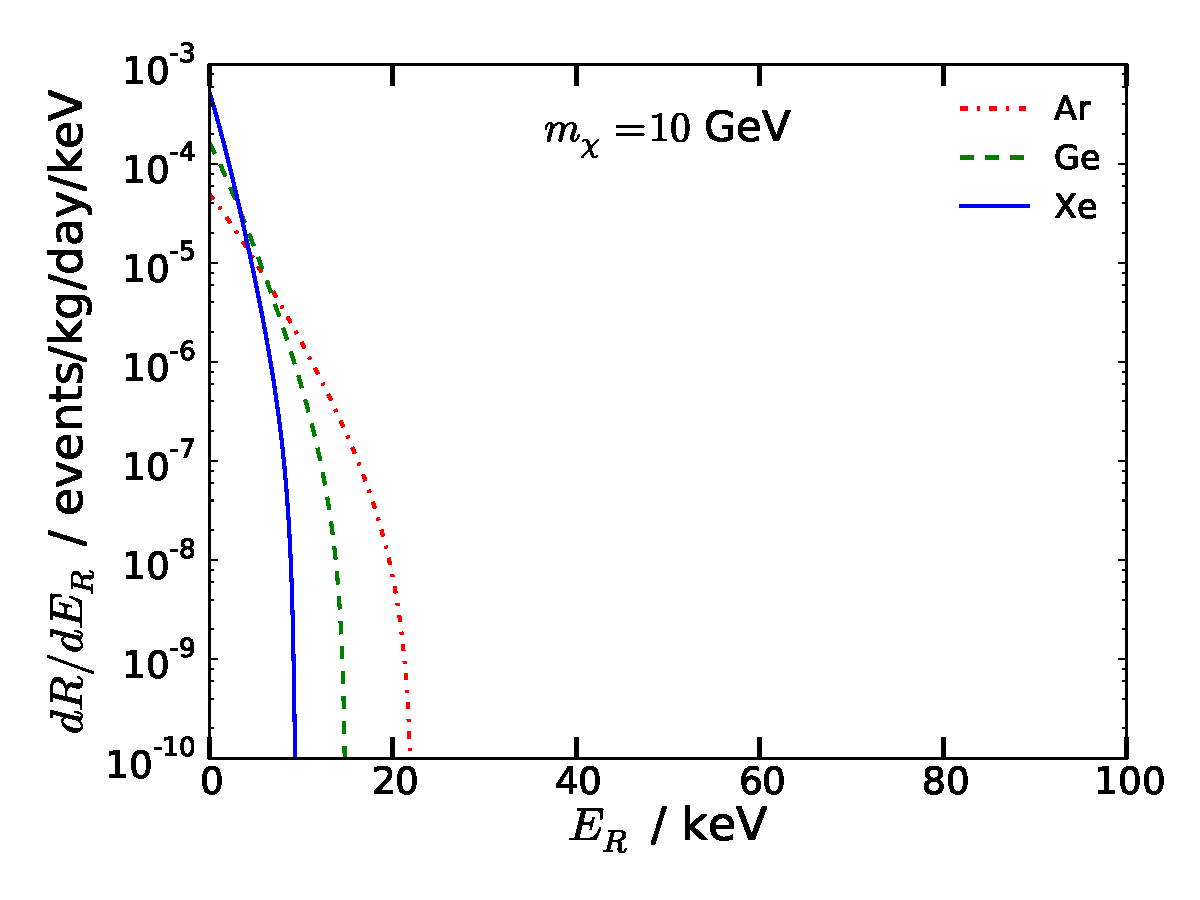
\includegraphics[width=0.75\textwidth]{DirectDetection/Spectra_10GeV.pdf}
  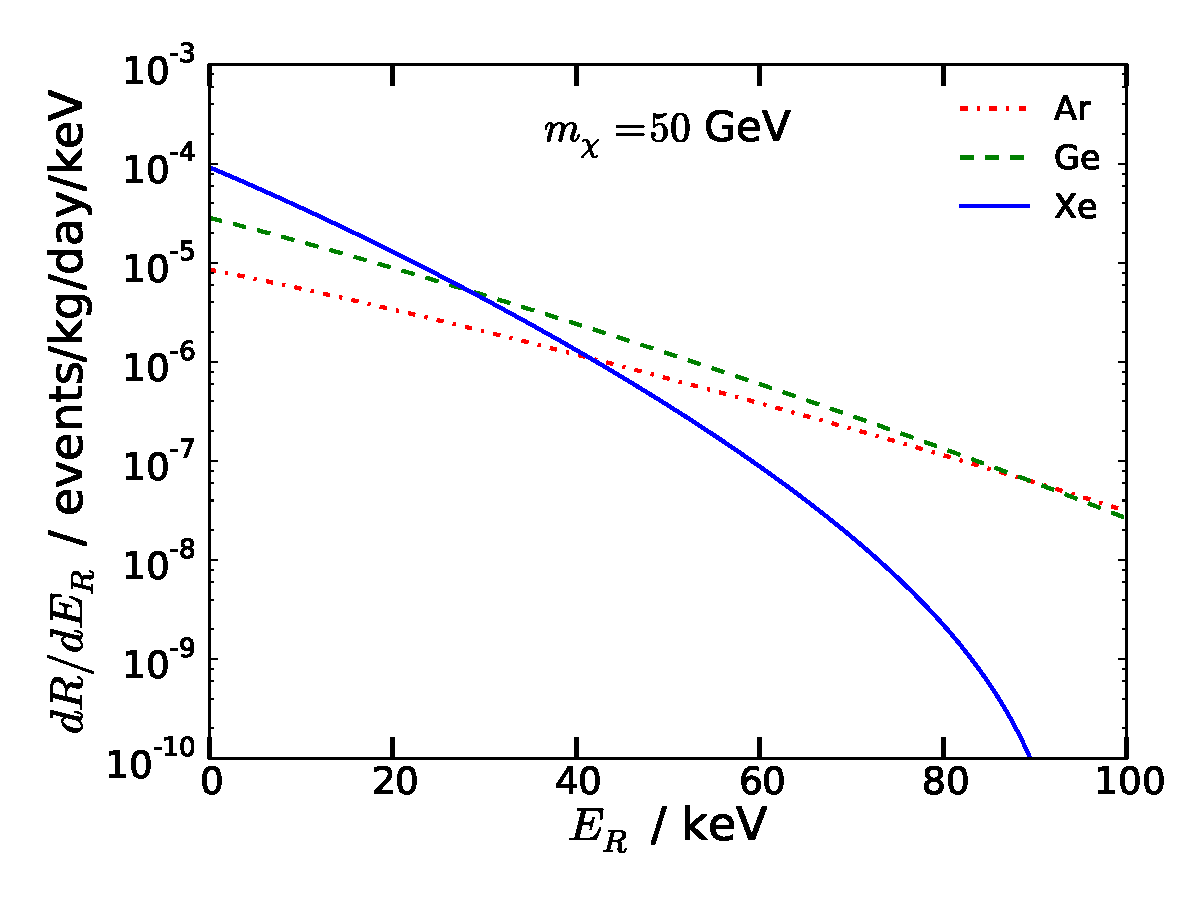
\includegraphics[width=0.75\textwidth]{DirectDetection/Spectra_50GeV.pdf}
  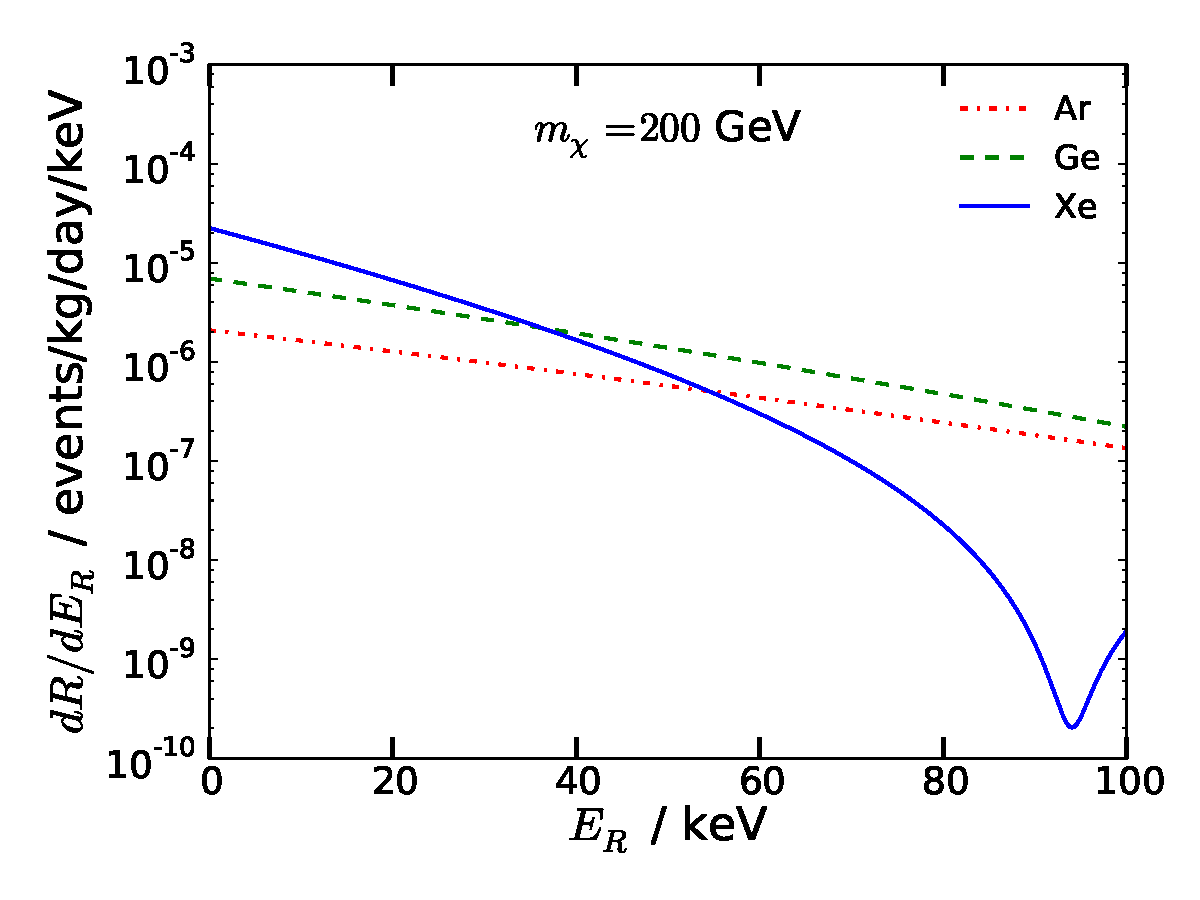
\includegraphics[width=0.75\textwidth]{DirectDetection/Spectra_200GeV.pdf}
  \caption[Examples of spin-independent event spectra for direct detection experiments]{Spin-independent differential event rates predicted for the nuclear targets Xenon (solid blue), Germanium (dashed green) and Argon (dot-dashed red) and for several WIMP masses $m_\chi$, assuming $f_p = f_n$. We assume a Standard Halo Model speed distribution, $\rho_0 = 0.3 \textrm{ GeV cm}^{-3}$ and a spin-independent cross section $\sigmapsi = 10^{-45} \textrm{ cm}^2$. The Helm form factor \cite{Helm:1956} is assumed (see Sec.~\ref{sec:DD:nuclearunc}).}
  \label{fig:DD:spectra}
\end{figure}

\begin{figure}[ht]
\centering
  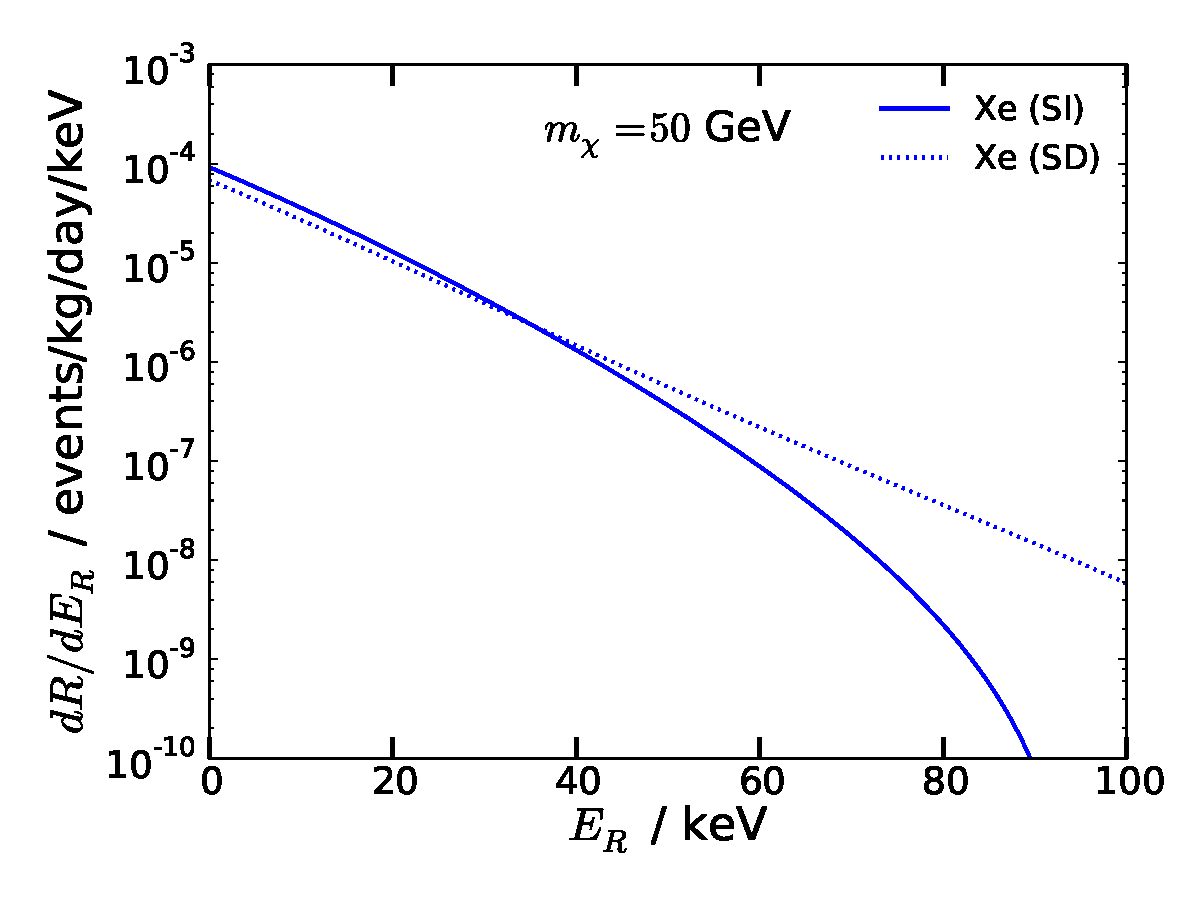
\includegraphics[width=0.75\textwidth]{DirectDetection/SpectraSISD_50GeV.pdf}
  \caption[Comparison of spin-dependent and spin-independent rates for a Xenon experiment]{Spin-dependent (dotted) and spin-independent (solid) differential event rates predicted for a Xenon nuclear target for a WIMP mass $m_\chi = 50 \textrm{ GeV}$, assuming $f_p = f_n$ and $a_p = a_n$. We assume a Standard Halo Model speed distribution, $\rho_0 = 0.3 \textrm{ GeV cm}^{-3}$ and cross sections $\sigmapsi = 10^{-45} \textrm{ cm}^2$ and $\sigmapsd = 10^{-40} \textrm{ cm}^2$. The Helm form factor \cite{Helm:1956} is assumed for the SI rate, while the SD form factor is taken from Ref.~\cite{Ressell:1997} using the NijmegenII calculation (see Sec.~\ref{sec:DD:nuclearunc}).}
  \label{fig:DD:spectraSISD}
\end{figure}


Finally, in Fig.~\ref{fig:DD:spectraSISD}, we show the SI and SD rates for a Xenon experiment and a WIMP mass of $m_\chi = 50 \textrm{ GeV}$. The SD rate gives a comparable contribution to the SI rate only with a cross section five orders of magnitude larger. This is due to the strong $A^2$ enhancement of the SI rate for heavy nuclei. For light nuclei such as Fluorine, the SI and SD rates will be closer in magnitude (for a given cross section). Figure~\ref{fig:DD:spectraSISD} also shows that the SD spectrum is typically flatter. The SD form factor has an approximately exponential form, while the SI form factor falls more rapidly (see Sec.~\ref{sec:DD:nuclearunc}). 

For a real experiment, the detector will be sensitive to recoil energies only in some range $E_\textrm{min}$ to $E_\textrm{max}$. The total number of events expected is obtained by integrating over this range of recoil energies and multiplying by the exposure time $t_\textrm{exp}$, detector mass $m_\textrm{det}$ and efficiency (which may also be a function of the recoil energy $E_R$) $\epsilon(E_R)$:

\begin{equation}
N_e = m_\textrm{det} t_\textrm{exp} \int_{E_\textrm{min}}^{E_\textrm{max}}\epsilon(E_R) \dbd{R}{E_R} \, \mathrm{d}E_R\,.
\end{equation}
For the case of a more realistic experiment in which the measurement of energy has only a finite resolution $\sigma(E_R)$, we convolve the event rate with a resolution function (which we assume to have a Gaussian form) to obtain the observed recoil spectrum $\mathrm{d}\tilde{R}/\mathrm{d}E_R$,
\begin{equation}
\dbd{\tilde{R}}{E_R}(E) = \int_{E' = 0}^{\infty} \frac{\mathrm{e}^{-(E - E')^2/(2\sigma(E'))}}{\sqrt{2\pi}\sigma(E')} \dbd{R}{E_R}(E') \, \mathrm{d}E'\,.
\end{equation} 

We now turn our attention to the discussion of such `realistic experiments' and the current state of dark matter direct searches. 



\section{Direct detection experiments}

%\note{Typical sources of backgrounds include \begin{inparaenum}[i)] \item $e/\gamma$ events, \item neutrons, \item $\alpha$-particles and \item nuclear recoils. \end{inparaenum}}



In order to measure the event spectrum, a range of obstacles must be overcome. One possible source of backgrounds are high energy cosmic rays. For this reason, direct detection experiments are typically operated underground, such as at the Gran Sasso laboratory in Italy or the Boulby laboratory in the UK, in order to reduce the penetration of these cosmic rays. However, cosmogenic muons and neutrons can still penetrate the experiments, leading to the need for active shields which can detect these particles and provide a veto for any nuclear recoils they produce. It is also possible to veto events which produce multiple-scatters in the detector as WIMPs are expected to scatter only once. Passive shielding also reduces the neutron flux from surrounding rock and other sources. For a detailed analysis of neutron sources at dark matter experiments, see Ref.~\cite{Scholl:2012} (CRESST-II) and Ref.~\cite{Aprile:2013b} (XENON100).

Radioactive decays due to naturally occuring isotopes may cause keV energy nuclear recoils in the detector, meaning that care must be taken to reduce their impact. The radiopurity of the target material is therefore of utmost importance (see for example Ref.~\cite{Munster:2014}), as well as the radiopurity of detector equipment itself \cite{Bernabei:2008b,Kuzniak:2012}. In some cases, the naturally occurring target material is contaminated with a particular radioisotope, such as $^{39}$Ar contamination in Argon. In these cases, special sources of the material must be found \cite{Galbiati:2008}, or the amount of contamination must be carefully monitored and reduced \cite{Abe:2009,Aprile:2013a}. 

A major source of backgrounds is also electron recoils, which deposit energy in the detector and must be distinguished from nuclear recoils caused by WIMP interactions. Depending on the design of the detector, different methods are used to discriminate electron from nuclear recoils and to measure the recoil energy itself. We will now summarise some of the techniques which are used.

%\note{Use \href{http://cdms.phy.queensu.ca/Public_Docs/DirectDetection.html}{this list}...}
%\todo{Say something about energy calibration and NR and EE...}
\todo{Which ones are sensitive to spin independent and spin dependent?}

Cryogenic experiments, such as CDMS \cite{Ahmed:2009,Ahmed:2011,Agnese:2013}, CRESST \cite{Angloher:2012}, CoGeNT \cite{Aalseth:2011a,Aalseth:2011b, Aalseth:2013,Aalseth:2014a,Aalseth:2014b} and EDELWEISS \cite{Armengaud:2011}, use cryogenic crystals of materials such as Germanium or Silicon as target materials. When a WIMP recoils from a target nucleus a phonons are generated in the crystal along with an ionization signal. By summing the energy collected in these two channels (and accounting for any which may be incompletely collected), the total energy of the nuclear recoil can be obtained. The ratio of the total nuclear recoil energy and the ionization signal is referred to as the `ionisation yield' and can be used to discriminate electron from nuclear recoils; electron recoils deposit more energy into ionisation. However, care must be taken to identify so-called `surface events' - events occurring close to the detector surface which result in an incomplete collection of ionisation signal and can thus mimic a WIMP signal.

Noble liquid experiments use liquid (or two-phase) noble elements such as Xenon and Argon as target materials. Completed or operational Xenon detectors include ZEPLIN \cite{Akimov:2012}, XENON \cite{Aprile:2011} and LUX \cite{Akerib:2014}. In these detectors, Xenon recoils produce a scintillation signal (S1) which can be observed directly using photomultiplier tubes. Ionisation electrons are also produced, which drift in an applied magnetic field, producing an electroluminescence signal (S2) in the gas phase. The sum of these signals can be used to reconstruct the total recoil energy, while the ratio S1/S2 is used to discriminate electron from nuclear recoils. The two signals can also be used to localise the event within the detectors. A fiducial volume is then defined within the detector - only events inside this volume are considered in data analysis. This allows liquid Noble detectors to be self-shielding; the fiducial volume is shielded by the remaining detector volume. Experiments utilising Argon \cite{Marchionni:2011, Badertscher:2013} and Neon \cite{Boulay:2008} are currently under development, using either the scintillation to ionisation signal as a discriminant or using timing of the scintillation signal (pulse shape discrimination).

Superheated liquid detectors such as COUPP \cite{Behnke:2011}, SIMPLE \cite{Felizardo:2012} and PICASSO \cite{Archambault:2012} use a detector volume filled with droplets of superheated liquid such as $\textrm{C}_4\textrm{F}_{10}$. The deposition of kinetic energy by a WIMP will induce the nucleation of a bubble producing an acoustic signal which is detected by piezoelectric transducers. Energy deposition by other particles such as muons and $\gamma$- and $\beta$-radiation typically occurs over longer length scales and thus does not register a signal. The temperature and pressure of the detector can be tuned to specify the threshold energy, the minimum energy which must be deposited before nucleation occurs. As such, superheated liquid detectors cannot measure the energy of specific events but rather the total event rate above the energy threshold. However, by ramping up the energy threshold, the recoil spectrum can effectively be measured. Due to the light targets such as Fluorine used by these experiments, they are typically more sensitive to light WIMPs with SD interactions.

Crystal scintillator experiments \cite{Kim:2010} such as DAMA/LIBRA \cite{Bernabei:2008a,Bernabei:2010,Bernabei:2013} and KIMS \cite{Lee:2007} use crystals such as Thallium-doped Sodium Iodide (NaI(Tl)) as the detector material. When a nuclear recoil occurs with the nuclei in the crystal, scintillation occurs. The light is collected by photomultiplier tubes, with the total recoil energy being related to the amount of scintillation light produced. In the case of DAMA/LIBRA, electron-nuclear recoil discrimination is not employed. Instead, the experiment aims to observe the annual modulation of the signal which is expected due to the periodic motion of the Earth through the WIMP halo. In other cases, such as NAIAD \cite{Ahmed:2003}, pulse shape discrimination has been used to distinguish nuclear and electronic recoils.

A final class of direct detection experiments are known as `directional' direct detection experiments. These aim to measure not only the energy deposited by WIMP scattering events but also the direction of the nuclear recoils. It is hoped that a recoil spectrum peaked in the direction opposite to the Earth's motion will provide strong evidence for a DM origin for the recoils. One possibility for this is the use of specialised gas time projection chambers (TPCs), which allow measurable track lengths from which the recoil direction can be determined. The directional detection of dark matter is the subject of Chapter~\ref{ch:Directional} and we defer a more detailed discussion of directional experiments until then.

\subsection{Current limits and results}

The first major dark matter detection to be reported was that of DAMA/NaI \cite{Bernabei:2003} and its successor DAMA/LIBRA. The experiments observed an annual modulation over 13 annual cycles, with a phase matching that expected from a dark matter signal. The detection of the annual modulation has been reported at the $8.9\sigma$ confidence level over an energy range of 2-6 keV. The modulation signal was only found in single-hit events at low energies, again suggesting a dark matter origin for the signal. It has been suggested that the signal may be explained by a dark matter particle of mass $m_\chi \sim 10 \textrm{ GeV}$ and SI cross section $\sigma_{SI} \sim 10^{-41} \textrm{ cm}^2$ \cite{Belli:2011} scattering off Sodium (or a heavier WIMP around 80 GeV scattering off Iodine \cite{Savage:2009}). An annual modulation signal was also observed in the CoGeNT experiment \cite{Aalseth:2011b, Aalseth:2014a}. In this case too, the period and phase are consistent with expectations, though, the amplitude of the annual modulation is approximately 5 times larger than expected. 

Excesses above the expected backgrounds have also been observed in a number of experiments.%including CoGeNT, CRESST-II and CDMS-Si. 
The CoGeNT experiment observed an exponentially rising excess of events at low energies, down to $0.5 \textrm{ keV}_{ee}$. A maximum likelihood analysis \cite{Aalseth:2014b} pointed towards a $10 \textrm{ GeV}$ WIMP interpretation, with a cross section of around $\sigma_{SI} \sim 5 \times 10^{-42} \textrm{ cm}^2$, though the significance of the `signal' lies at only 2.9$\sigma$. CRESST-II \cite{Angloher:2012} observe 67 events in the nuclear recoil signal region but expect a background of only one event due to leakage of electron recoils into this window. Taking into account other backgrounds, the CRESST-II collaboration estimate that 25-30 of these events may be due to a WIMP signal. A fit to the data produces two minima in the likelihood function: one at $m_\chi \approx 25 \textrm{ GeV}$ (in which scattering from Tungsten is appreciable) and another at $m_\chi \approx 12 \GeV$ (where Tungsten recoils lie below the energy threshold). In both cases, the fitted cross section is in the range $\sigma_{SI} \approx 10^{-42} - 5 \times 10^{-41} \textrm{ cm}^2$. Finally, a recent analysis of the Silicon detector data from CDMS-II  \cite{Agnese:2013} finds 3 events in the signal region. However, the very low expected backgrounds mean that this small number of events may be significant. The probability of the known backgrounds producing these three events has been calculated at 5.4\% and a likelihood analysis shows consistency with WIMP with $m_\chi \approx 9 \GeV$ and $\sigma_{SI} \approx 2 \times 10^{-41} \cmsq$.

While it appears that a reasonably consistent picture of a low mass WIMP is emerging from several experiments \cite{Hooper:2010}, a large number of competing experiments have reported null results. Results from CDMS-II (Ge), XENON100, LUX, SuperCDMS \cite{Agnese:2014} and others set upper limits on the standard WIMP cross section several orders of magnitude lower than the claimed signal. Several explanations for this discrepancy have been offered. One possibility is background contamination of the experiments claiming to have observed a signal, which has been suggested in the case of CRESST-II \cite{Kuzniak:2012}. A recent analysis of the CoGeNT excess \cite{Davis:2014} find evidence for DM at less than $1\sigma$ using an improved method for rejecting surface events. In the case of DAMA/LIBRA, it has been suggested that ion-channeling in the detector crystals may affect the collected ionisation signal and therefore alter the signal \cite{Bozorgnia:2010}. The DAMA/LIBRA signal has also been attributed to an annually modulated muon signal \cite{Blum:2011,Bernabei:2012}.

An alternative explanation is that the claimed signals \textit{are} due to a dark matter particle, but that its properties are not as simple as in the canonical case, explaining why it has not been observed in all experiments. One possibility is that the astrophysical distribution of dark matter does not match the standard assumptions. We will discuss this astrophysical distribution in more detail shortly in Sec.~\ref{DD:sec:astrounc}. However, it appears that even with this additional freedom, the different results cannot be reconciled \cite{Fairbairn:2009,Herrero-Garcia:2012,Fox:2011b,Frandsen:2012}. A number of particle physics models have also been considered to explain the results, including spin-dependent interactions \cite{Buckley:2013}, isospin violating dark matter (for which $f^p \neq f^n$) \cite{Feng:2011}, inelastic dark matter \cite{Smith:2001} and mirror dark matter \cite{Foot:2013}. However, a consistent picture which reconciles all experimental datasets remains elusive \cite{Schwetz:2011}. %\note{IVDM is invoked to reduce sensitivity to a particular experiment...}

We summarise some of the completed and current direct detection experiments in Table~\ref{DD:tab:ExptSummary}. The most stringent limits on the SI WIMP-proton cross section are set by LUX \cite{Akerib:2014}, who find a limit of $\sigma_{SI}^p \leq 7.6 \times 10^{-46} \cmsq$ at a mass of $m_\chi = 33 \GeV$. The best limit for the SD cross section is set by XENON100 \cite{Aprile:2013c}: $\sigma_{SD}^p \leq 3.5 \times 10^{-40} \cmsq$. The confirmation or falsification of the signals which have been claimed thus far may have to wait for the next generation of dark matter experiments, or for corroboration from collider or indirect searches. 


\begin{table}
	\begin{tabular}{ccc}
		%Give references to results and 'setup'papers...
		\hline\hline
		Experiment & Target & Status \\
		\hline
		CDMS-II (Ge) \cite{Ahmed:2009,Ahmed:2011} & Ge & Null result \\
                CDMS-II (Si) \cite{Agnese:2013} & Si & Excess \\
                SuperCDMS \cite{Agnese:2014} & Ge & Null result \\
		CoGeNT \cite{Aalseth:2011a,Aalseth:2011b, Aalseth:2013,Aalseth:2014a,Aalseth:2014b} & Ge & Excess \& annual modulation\\
		CRESST-II \cite{Angloher:2012} & CaWO\(_4\) & Excess\\
		EDELWEISS-II \cite{Armengaud:2011} &  Ge & Null result \\
		ZEPLIN-III \cite{Akimov:2012} & Xe & Null result\\
		XENON100 \cite{Aprile:2011, Aprile:2012b} & Xe & Null result \\
                LUX \cite{Akerib:2014} & Xe & Null result \\
		PICASSO \cite{Archambault:2012} & \(\textrm{C}_4\textrm{F}_{10}\) & Null result \\
		SIMPLE-II \cite{Felizardo:2012} & \(\textrm{C}_2 \textrm{ClF}_5\) & Null result \\
		COUPP \cite{Behnke:2011} & CF\(_3\)I & Null result \\
		DAMA/LIBRA \cite{Bernabei:2008a,Bernabei:2010,Bernabei:2013} &  NaI(Tl) & Annual modulation\\
                NAIAD \cite{Ahmed:2003} & NaI(Tl) & Null result \\
		KIMS \cite{Lee:2007} & CsI(Tl) & Null result \\
		\hline\hline
		\end{tabular}
	\caption{Summary of current and completed direct detection experiments.}
	\label{DD:tab:ExptSummary}
\end{table}


\todo{TEXONO \cite{Li:2013}}

\todo{Give some typical values for thresholds and efficiencies..?}

\begin{comment}
\begin{figure}[h]
  \centering
  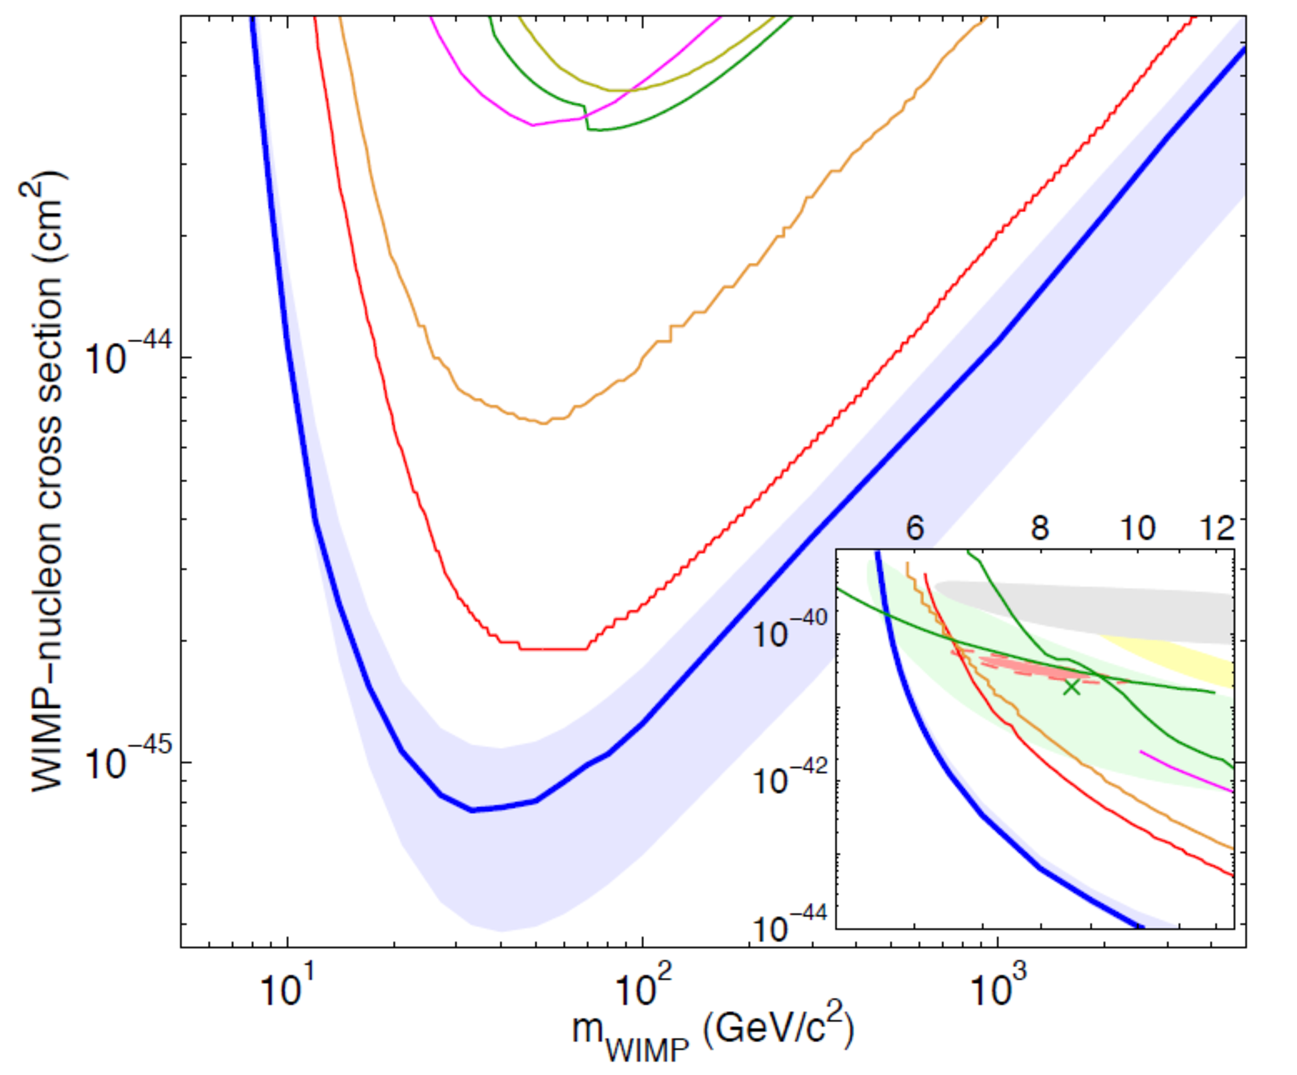
\includegraphics[width=0.75\textwidth]{DirectDetection/SIlimits.pdf}
  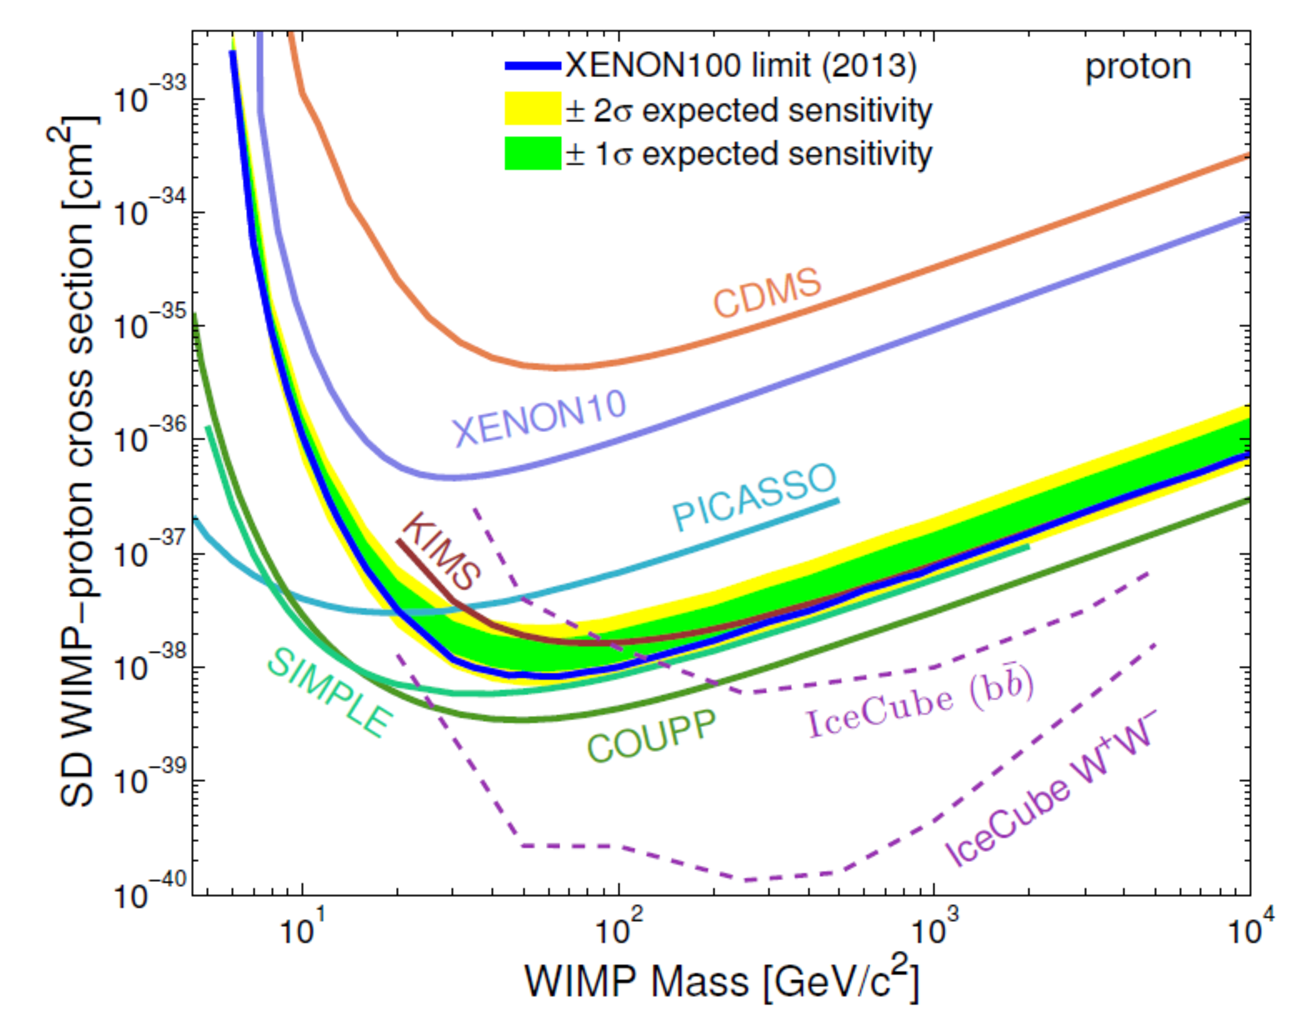
\includegraphics[width=0.75\textwidth]{DirectDetection/SDlimits.pdf}
  \caption[]{}
  \label{fig:DD:CurrentLimits}
\end{figure}
\end{comment}

\subsection{Future experiments}

Experiments which are planned or under construction typically aim to scale up the size of current detectors and reduce unwanted backgrounds (in order to increase the sensitivity to lower cross sections) or decrease the energy threshold (which increases sensitivity to lower masses). There are a number of ton scale detectors either in operation or planned, including XENON1T \cite{Aprile:2012a}, DEAP-3600 \cite{Gorel:2014}, LZ \cite{Malling:2011}, EURECA \cite{Kraus:2007,Roth:2009} and DARWIN \cite{Baudis:2012}. With this next generation of detectors, the aim is to achieve sensitivity to the SI WIMP-proton cross section down to $\sigma_{SI}^p = 10^{-48} \cmsq$. Below this value, irreducible backgrounds from neutrinos (predominantly from the Sun) become important and the identification of a DM signal becomes more difficult \cite{Monroe:2007,Billard:2014}.


There have also been a number of proposals for novel methods of directly detecting dark matter. These include using DNA-based detectors to provide high spatial resolution \cite{Drukier:2012}, using nano-scale explosives \cite{Lopez:2014} or charged-coupled devices \cite{Aguilar-Arevalo:2013} to achieve very low energy thresholds and using proton-beam experiments as a source for dark matter source for direct detection experiments \cite{deNiverville:2012}.

%\todo{Mini-conclusion...}

\todo{What about electron recoils...?}

\section{Uncertainties}

Calculation of the DM differential event rate $\mathrm{d}R/\mathrm{d}E_R$ requires not only a knowledge the dark matter parameters $m_\chi$ and $\sigma_{SI,SD}$ but a number of other factors which also enter into the calculation. It is important to understand how uncertainties in these different factors and parameters propagates into the event rate in order to ensure that the conclusions we draw from direct detection experiments are unbiased. These uncertainties are typically partitioned into three separate classes: nuclear physics, particle physics and astrophysics.

\subsection{Nuclear physics uncertainties}
\label{sec:DD:nuclearunc}

As we have already seen, nuclear physics enters into the calculation of the nucleon matrix elements $m_n f_{Tq}^n \equiv \langle n|m_q\bar{q}q|n \rangle$. The factors $f_{Tq}^n$ must be determined experimentally, and have values

\begin{equation}
f_{Tu}^p = 0.020 \pm 0.004 ;\, f_{Td}^p = 0.026 \pm 0.005 ;\, f_{Ts}^p = 0.118 \pm 0.062\,,
\end{equation}
with $f_{Tu}^p = f_{Td}^n$, $f_{Td}^p = f_{Tu}^n$ and $f_{Ts}^p = f_{Ts}^n$. %\note{Strange content is most important - justifying fp = fn...?} 
The main uncertainties stem from determinations of the $\pi$-nucleon sigma term, determined either experimentally from low energy pion-nucleon scattering \cite{Borasoy:1995, Pavan:2001,Alarcon:2012} or from lattice QCD calculations \cite{Bali:2012, Alvarez-Ruso:2014}. Similarly for the spin contributions $\Delta_q$ to the nucleus, values must be obtained experimentally \cite{Ashman:1988,Jaffe:1990,Engel:1992,Adams:1997},

\begin{equation}
\Delta_u^p = 0.77 \pm 0.08 ;\, \Delta_d^p = -0.38 \pm 0.08 ;\, \Delta_s^p = -0.09 \pm 0.08\,,
\end{equation}
although efforts are being made to obtain these values directly via calculation \cite{Qing:1998,Thomas:2008}. It should be noted that these nucleon matrix elements are only necessary if we wish to deal directly with quark-level couplings and interactions. If, instead, we consider the nucleon-level effective operators (and equivalently the WIMP-nucleon cross sections), these values are not required. %\note{Is this from muon-proton scattering?}

Nuclear physics also enters into the calculation of form factors, describing the internal nucleon and spin structures of the nuclei. For the SI case, the form factor is obtained from the Fourier transform of the nucleon distribution in the nucleus. The form typically used is due to Helm \cite{Helm:1956}

\begin{equation}
F_{SI}^2(E_R) = \left(\frac{3j_1(qR_1)}{qR_1}\right)^2 \mathrm{e}^{-q^2s^2}\,,
\end{equation}
where $j_1(x)$ is a spherical bessel function of the first kind,
\begin{equation}
j_1(x) = \frac{\sin x}{x^2} - \frac{\cos x}{x}\,.
\end{equation}
Nuclear parameters due to Lewin and Smith \cite{Lewin:1996}, based on fits to muon spectroscopy data \cite{Fricke:1995} are typically used:
\begin{align}
R_1 & = \sqrt{c^2 + \frac{7}{3}\pi^2a^2 - 5s^2}, \\
c & = 1.23A^{1/3} - 0.60 \mathrm{ fm}, \\
a & = 0.52 \mathrm{ fm}, \\
s & = 0.9 \mathrm{ fm} \,.
\end{align}
Muon spectroscopy and electron scattering data \cite{Duda:2007} are typically used as a probe of the \textit{charge} distribution in the nucleus. However, detailed Hartree-Fock calculations indicate that the charge distribution can be used as a good proxy for the nucleon distribution (especially in the case $f_p \approx f_n$) and that using the approximate Helm form factor introduces an error of less than $\sim$5\% in the total event rate \cite{Co:2012}. Studies also indicate that errors due to distortions in nuclear shape away from sphericity are negligible \cite{Ya-Zheng:2012}.

%\todo{Include a table of Sp and Sn values - or values for N, alpha, beta - table in \cite{Jungman:1995}}
In the SD case, however, the situation is more complicated. In order to calculate the SD cross section, we require the proton and neutron spin content $\langle S_{p,n} \rangle$ as well as the form factor $F_{SD}^2$. The form factor can be written in the form

\begin{equation}
F_{SD}^2(E_R) = S(E_R)/S(0)\,,
\end{equation}
in terms of the response function $S(E_R)$. This response function can in turn be decomposed into three spin-dependent structure functions (SDSFs)

\begin{equation}
S(E_R) = a_0^2S_{00}(E_R) + a_0a_1S_{01}(E_R) + a_1^2S_{11}(E_R)\,,
\end{equation}
where $a_0 = a_p + a_n$ is the isoscalar coupling and $a_1 = a_p - a_n$ is the isovector coupling. The zero momentum transfer value $S(0)$ is related to the proton and neutron spin expectation values by \cite{Cannoni:2013}
\begin{equation}
S(0) = \frac{2J + 1}{\pi} \frac{J+1}{J} \left|a_p\langle S_p \rangle + a_n \langle S_n \rangle\right|^2\,.
\end{equation}
We can therefore rearrange the SD cross section of Eq.~\ref{DD:eq:sigsd} as

\begin{equation}
\dbd{\sigma_{SD}}{E_R} = \frac{2\pi}{3} \frac{m_N \sigma_{SD}^p}{\mu_{\chi p}^2 v^2} \frac{1}{2J+1} \frac{S(E_R)}{(a_p)^2}\,.
\end{equation}
The nuclear physics is now encapsulated in a single response function $S(E_R)$ (or equivalently two SDSFs $S_{00}$ and $S_{11}$).\footnote{In Ref.~\cite{Cannoni:2013}, it is noted that the SDSFs are not independent and that the function $S_{01}$ can be written in terms of the other two.}

The functional form for $S_{ij}$ can be calculated from shell models for the nucleus \cite{Ressell:1997}. However, there are a number of competing models (such as the Odd Group Model \cite{Engel:1989}, Interacting Boson Fermion Model \cite{Iachello:1991} and Independent Single Particle Shell Model \cite{Ellis:1988} among others). These models use different methods for accounting for forces between quarks, leading to different forms for the SDSFs and therefore to significant uncertainty in the spin-dependent cross section. This issue was explored by Cerde\~{n}o \etal \cite{Cerdeno:2012}, who developed a parametrisation for the spin structure functions in terms of the parameter $u = (qb)^2/2$, where $q$ is the momentum transfer and $b = \sqrt{41.467/(45.0 A^{-1/3} - 25.0 A^{-2/3})}$ is the oscillator size parameter. This parametrisation takes the form

\begin{equation}
\label{eq:SDparametrisation}
S_{ij} = N ((1-\beta)\mathrm{e}^{-\alpha u} + \beta)\,,
\end{equation}
where the range of the parameters $\left\{N, \alpha, \beta\right\}$ is chosen such that $S_{ij}$ spans the different possible forms presented in the literature. It was shown that this parametrisation was able to mitigate the uncertainties in the SD cross section and accurately recover the remaining particle physics parameters when the true form for the SDSFs was unknown.

\subsection{Particle physics uncertainties}
\label{sec:DD:particleunc}
Apart from the unknown values for the WIMP mass $m_\chi$ and cross sections $\sigma_{SI,SD}$, the ratios of proton to neutron couplings are also \textit{a priori} unknown. In the case of SI scattering, the dominant contribution comes from the coupling to strange quarks $f_{Ts}$, which is equal for protons and neutrons. It is therefore typically assumed that $f^p = f^n$, though isospin violating dark matter models have been considered \cite{Feng:2011, Kumar:2012,Hamaguchi:2014}. Similarly, for the SD interaction, a specific relation is typically assumed between the proton and neutron couplings, such as $a_p/a_n = \pm1$. While specific models often predict such a relation \cite{Jungman:1995}, it should be noted that this ratio is \textit{a priori} unknown and fixing it is a model choice.

Further uncertainty is derived from the form of the interaction terms themselves. Here, we have considered the dominant contributions to scattering in the case of non-relativistic contact interactions. Extensions including mediator particles have been considered \cite{Schmidt-Hoberg:2013, An:2014}, as well as models in which DM can interact electromagnetically with nuclei \cite{Pospelov:2000, Ho:2013}. There has also been significant effort towards developing a general non-relativistic field theory for the interaction of WIMPs with nuclei \cite{Kurylov:2003,Fan:2010,Cirelli:2013,Fitzpatrick:2013}. Current limits can be translated into limits on the couplings associated with a range of effective operators. While this approach significantly widens the parameter space of dark matter direct detection, it is more general and does not rely on (potentially poor) assumptions about DM interactions.

%\note{Asymmetric DM?}

\subsection{Astrophysical uncertainties}
\label{sec:DD:astrounc}

Astrophysical uncertainties enter into the direct detection event rate through the local dark matter density $\rho_0$ and the speed distribution $f_1(v)$. 

\subsubsection{DM density, $\rho_0$}

The DM mass density sets the overall scale of the scattering rate. As we shall discuss in Chapter~\ref{ch:Speed}, the DM density is degenerate with the interaction cross section, meaning that an accurate determination is important. One method of obtaining the value of $\rho_0$ is by mass modelling of the Milky Way (MW). One builds a model for the Galaxy incorporating various sources of mass, including the stellar bulge and disc, dust and a dark matter halo \cite{Catena:2010}. It is then possible to use various data such as the total MW mass, local surface mass density and the velocities of tracers to fit the parameters of this model and thereby extract $\rho_0$. Estimates using this method tend to have a wide uncertainty, typically lying in the range \(0.2 - 0.4 \textrm{ GeV cm}^{-3}\) (e.g.\ Ref.\ \cite{Catena:2010,Weber:2010}). A more recent determination using state-of-the-art data obtains a more precise but higher value of $\rho_0 = 0.47_{-0.06}^{0.05} \textrm{ GeV cm}^{-3}$ \cite{Nesti:2013} (though this depends on the choice of halo density profile). 

An alternative method is to use local stellar kinematic data to constrain the gravitational potential near the Sun and thus obtain an estimate of $\rho_0$. Using kinematic data from roughly 2000 K-dwarfs, Garbari \etal \cite{Garbari:2012} obtain the value \(\rho_0 = 0.85_{-0.50}^{+0.57} \textrm{ GeV cm}^{-3}\) while Zhang \etal, using a larger sample of 9000 K-dwarfs, obtain $0.28\pm0.08 \textrm{ GeV cm}^{-3}$. Including microlensing data, the range of allowed values at $1\sigma$ is $\rho_0 = 0.20-0.56 \textrm{ GeV cm}^{-3}$ \cite{Iocco:2011}. A further model independent method was proposed by \cite{Salucci:2010}. The advantage of such approaches is that one does not need to assume a particular form for the DM halo density profile. However, they may be more sensitive to assumptions about local equilibrium near the Sun's position.

In 2012, Moni Bidin \etal \cite{Moni-Bidin:2012} used the dynamics of thick disk stars to constrain the DM density, finding a result consistent with no dark matter at the Sun's radius. However, a subsequent reanalysis by Bovy and Tremaine \cite{Bovy:2012} showed that this result derived from a poor assumption about the velocity of stellar tracers as a function of Galactic radius. Using the same data with more reasonable assumptions, the value $0.3 \pm 0.1 \textrm{ GeV cm}^{-3}$ was obtained. 

In spite of the large number of determinations, no consistent value appears to be emerging, with values ranging from $0.2 - 0.85 \textrm{ GeV cm}^{-3}$ . There also remain a number of uncertainties in these determinations, including the shape of the DM halo and assumptions about the local equilibrium of the Galaxy (for a recent review, see Ref.~\cite{Read:2014}). The `standard' value assumed in the analysis of direct detection experiments is $0.3 \textrm{ GeV cm}^{-3}$, though the exact origin of this number is unclear \cite{Green:2012}. 

\subsubsection{Speed distribution, $f_1(v)$}

The speed distribution enters into the direct detection rate in the integral,

\begin{equation}
\eta(v_\textrm{min}) \equiv \int_{v_\textrm{min}}^\infty \frac{f_1(v)}{v} \, \mathrm{d}v\,,
\end{equation}
which is referred to as the `velocity integral' or the `mean inverse speed'. Direct detection experiments are traditionally analyzed within the framework of the Standard Halo Model (SHM), in which WIMPs are assumed to have a Maxwell-Boltzmann velocity distribution in the Galactic frame. In the Earth's frame, this takes the form 

\begin{equation}
\label{eq:gaussian}
f_{\textrm{SHM}}(\textbf{v}) = N \exp\left(-\frac{(\textbf{v} - \textbf{v}_\textrm{lag})^2}{2\sigma_v^2}\right) \Theta(v_\textrm{esc} - |\textbf{v} - \textbf{v}_\textrm{lag}|)\,,
\end{equation}
where $\textbf{v}_\textrm{lag}$ specifies the velocity of the Earth frame with respect to the Galactic rest frame and $\sigma_v$ the velocity dispersion. The SHM distribution is obtained assuming a spherical, isothermal DM halo with density profile $\rho \sim r^{-2}$ and results in the relation $\sigma_v = v_\textrm{lag}/\sqrt{2}$. The distribution is truncated above the escape speed $v_\textrm{esc}$ in the Galactic frame and the factor $N$ is required to satisfy the normalization condition:

\begin{equation}
\label{eq:DD:normalization}
\int f(\textbf{v}) \, \mathrm{d}^3\textbf{v} = 1\,.
\end{equation}
By integrating over directions we obtain $f(v)$ and the speed distribution is then given by

\begin{equation}
f_1(v) = f(v) v^2 = \int f(\textbf{v}) v^2 \, \mathrm{d}\Omega_v\,. 
\end{equation} 

Within the SHM, there is some uncertainty on the parameters describing $f_1(v)$. The parameter $v_\textrm{lag}$ is given by the local circular speed $v_c = 218 \pm 7 \kms$ \cite{Kerr:1986,Feast:1997} plus a contribution from the peculiar motion of the Sun and the Earth's orbital motion. This lag speed is typically assumed to be close to the local circular speed, though more recent determinations of the solar velocity point towards higher values \cite{Schonrich:2012,Bovy:2012a} of $240-250 \kms$. The Galactic escape velocity can be estimated from the radial velocities of MW stars; the RAVE survey obtain the range $v_\textrm{esc} = 533_{-41}^{+54} \kms$ at 90\% confidence \cite{RAVE:2007, RAVE:2014}. Moreover, the relation $\sigma_v =  v_\textrm{lag}/\sqrt{2}$ is obtained from solving the Jeans equation assuming $\rho \sim r^{-2}$ \cite{Binney:2008}. Relaxing this assumption means that this relation no longer holds and that $\sigma_v$ is no longer as well constrained. 

Even taking into account these uncertainties, the SHM is unlikely to be an accurate representation of the DM halo. Observations and N-body simulations indicate that the halo should deviate from a $1/r^2$ profile and may not be spherically symmetric. As a result alternative models have been proposed. Speed distributions associated with triaxial halos \cite{Evans:2000} or with more realistic density profiles \cite{Widrow:2000} have been suggested, as well as analytic parametrisations which should provide more realistic behaviour at low and high speeds \cite{Lisanti:2010}. Self-consistent distribution functions reconstructed from the potential of the Milky Way have also been obtained \cite{Bhattacharjee:2012,Fornasa:2013}.

It is also possible to extract the speed distribution from N-body simulations. Such distribution functions tend \cite{Vogelsberger:2009, Kuhlen:2010, Mao:2012} to peak at lower speeds than the SHM and have a more populated high speed tail. There are also indications that DM substructure may be significant, causing `bumps' in the speed distribution, or that DM which has not completely phase-mixed - so-called `debris flows' - may have a contribution \cite{Kuhlen:2012}. \note{Show a plot?}

 It should be noted that N-body simulations do not probe down to the sub-milliparsec scales which are probed by direct detection experiments. There may be a concern then that the local dark matter distribution could be dominated by localised subhaloes or streams which are not captured by these simulations and which may affect the interpretation of direct detection experiments \cite{Freese:2004}. However, an analysis of N-body simulations has found that no individual subhalos should dominate the local distribution \cite{Helmi:2002}. Vogelsberger \etal \cite{Vogelsberger:2007} study the geodesic deviation of individual particles in N-body simulations, giving access to information about the ultra-local DM distribution. They find that the local distribution should be made up of a large number of streams ($\sim 10^5$), meaning that it can effectively be treated as smooth.

%This means that N-body speed distributions are averaged over large volumes in order to obtain sufficient statistics. The effect of probing the speed distribution over such large length scales (rather than on the ultra local scale of experiments) is not known.
%So far, we have assumed that dark matter in the Sun's vicinity is smoothly distributed. The possibility that some of the DM density is contributed by localised subhaloes or streams which have not reached equilibrium may affect the interpretation of direct detection experiments \cite{Freese:2004}. However, an analysis of N-body simulations has found that no individual subhalos should dominate the local distribution \cite{Helmi:2002}. Vogelsberger \etal \cite{Vogelsberger:2007} study the geodesic deviation of individual particles in N-body simulations, allowing them to access information about the ultra-local DM distribution. They find that the local distribution should be made up of a large number of streams ($\sim 10^5$) and can effectively be treated as smooth.

Another result obtained from N-body simulations is the possibility of a dark disk. When baryons are included in simulations of galaxy formation, this results in the tidal distruption of DM subhaloes which are then preferentially dragged into the disk plane \cite{Read:2009, Read:2010}. The resulting dark disk corotates with approximately the same speed as the baryonic matter, though with a smaller velocity dispersion $\sigma_v^{DD} \sim 50 \kms$. This dark disk is expected to contribute an additional density 0.2-1.0 times the density of the halo. However, this value is dependent on the merger history of the Milky Way, with more massive and numerous mergers leading to an enhance disk density. The more recent ERIS results \cite{Pillepich:2014}, comparing hydrodynamic and DM-only simulations, report a relatively quiet merger history for a Milky Way-like galaxy. The result is a smaller dark disk density of just 10\% that of the DM halo.

In Fig.~\ref{fig:DD:SpeedDists}, we show some examples of possible dark matter speed distributions in the Earth frame. We show the directionally averaged velocity distribution $f(v)$ in the top panel, the speed distribution $f_1(v)$ in the middle panel and the corresponding $\eta(v)$ in the bottom panel. The population of low speed WIMPs in the SHM + dark disk (dashed green) distribution causes the mean inverse speed (and therefore the event rate) to rise more rapidly at low speeds than the SHM alone (solid blue). A sharp stream distribution function (dotted magenta) leads to step-like form for $\eta$; for $\vmin$ above the speed of the stream almost no WIMPs can contribution to the scattering, while for $\vmin$ below the speed of the stream almost all can. Each of these possible distributions will produce a different event spectrum in a detector.

\todo{Say something about monotonically decreasing...}


The impact of such uncertainties in the WIMP speed distribution has been much studied (see e.g.\ Refs.~\cite{Green:2010, Peter:2011, Fairbairn:2012}) and it has been shown that poor assumptions about the speed distribution may result in biased reconstructions of the DM mass and cross sections from future direct detection data. It is unknown which, if any, of the many distributions discussed here best describes the true Galactic DM speed distribution. It is therefore imperative that we model the uncertainties in $f_1(v)$ in a general way. Chapter~\ref{ch:Speed} addresses the various attempts to achieve this in the literature and explores what is required for such a general approach. 


\begin{figure}[h]
  \centering
  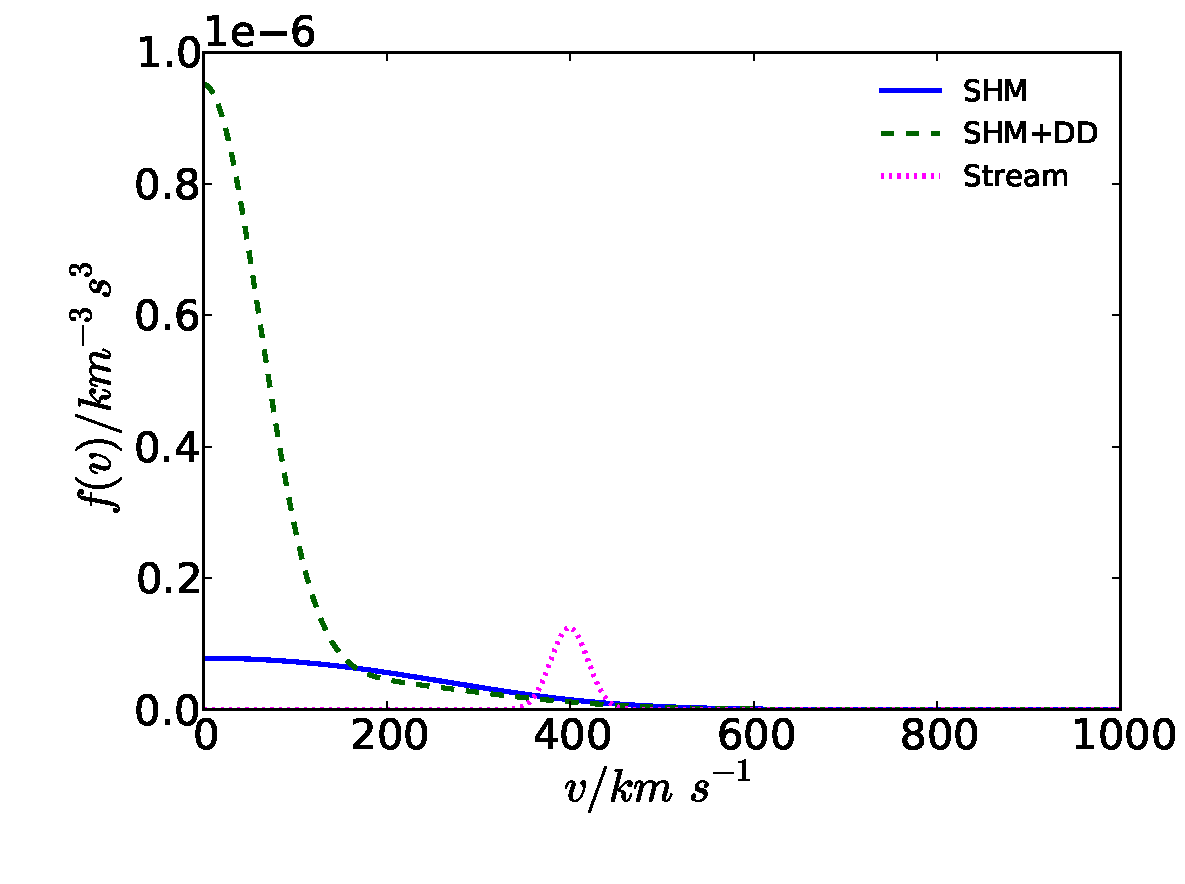
\includegraphics[width=0.75\textwidth]{DirectDetection/f.pdf}
  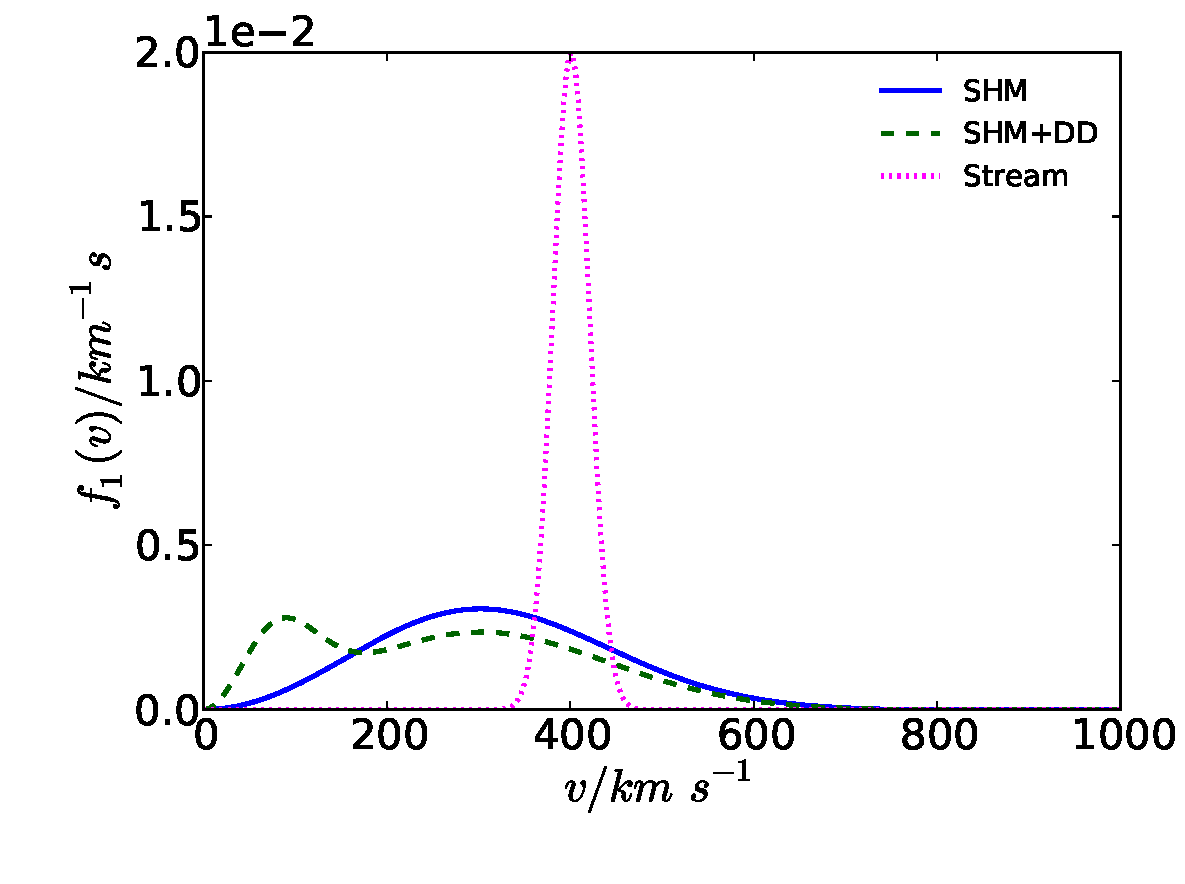
\includegraphics[width=0.75\textwidth]{DirectDetection/f1.pdf}
  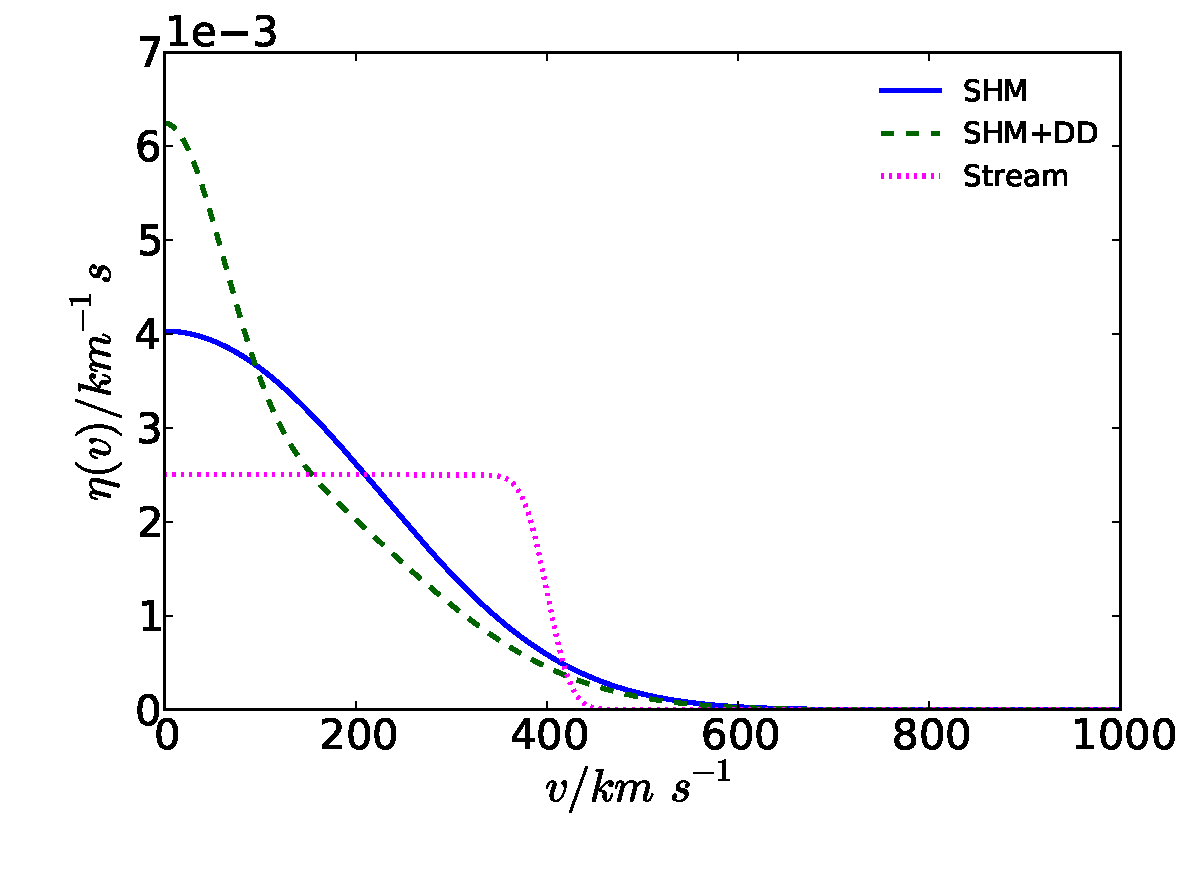
\includegraphics[width=0.75\textwidth]{DirectDetection/eta.pdf}
  \caption[Examples of dark matter speed distributions]{Some examples of possible dark matter speed distributions including the Standard Halo Model (SHM), SHM with a 30\% dark disk overdensity (SHM+DD), and a stream centred around $400 \kms$. We show the directionally averaged velocity distribution $f(v)$ (top panel), the speed distribution $f_1(v)$ (middle panel) and mean inverse speed $\eta(v)$ (bottom panel). }
  \label{fig:DD:SpeedDists}
\end{figure}

\begin{comment}
A first step is to extend the SHM to incorporate uncertainties in $v_\textrm{lag}$, $\sigma_v$ and $v_\textrm{esc}$ into reconstructions. Strigari and Trotta \cite{Strigari:2009} introduce a simple model of the Milky Way mass distribution, from which SHM velocity parameters can be derived. They then use projected stellar kinematics and direct detection data to fit both the model parameters and the dark matter properties. A more direct approach is to directly fit the SHM velocity parameters, incorporating their uncertainties into the fitting likelihood. This method has been considered by Peter \cite{Peter:2010}, and is typically used as a simple model of astrophysical uncertainties (especially in studies which focus on other aspects of direct detection, e.g.\ Ref.~\cite{Arina:2013}). These methods allow bias in the reconstructed WIMP parameters to be eliminated when the underlying speed distribution is indeed in the SHM form. However, as shown by Peter \cite{Peter:2011}, these methods fail when the distribution function differs from the standard Maxwellian case.

There have also been attempts to incorporate and fit more realistic distribution functions. Pato et al. \cite{Pato:2011} incorporate astrophysical uncertainties by using the distribution function of Lisanti et al. \cite{Lisanti:2010} and fitting the various shape parameters associated with it. In a more recent paper, Pato et al. \cite{Pato:2013} use projected direct detection data to fit a model of the Milky Way mass distribution, from which they derive a self-consistent distribution function (SCDF) using Eddington's formula. This means that the resulting speed distribution will be consistent with the underlying potentials of the galaxy's bulge, disk and dark matter, incorporating a broader range of shapes than the SHM alone. However, as the authors point out, velocity distributions from cosmological N-body simulations differ significantly from those expected from Eddington's formula. As with the Standard Halo Model, fitting a realistically-motivated distribution function is likely to result in biased reconstructions if the true distribution deviates significantly from the functional form used for fitting.

Methods which make no assumptions about the functional form of the speed distribution have had mixed success. Drees and Shan \cite{Drees:2007, Drees:2008} developed a method for estimating the WIMP mass by calculating moments of the speed distribution. However, this method still introduces a bias into the reconstructed WIMP mass and performs more poorly for heavier WIMPs and when finite energy thresholds are considered. An empirical ansatz for the speed distribution has also been suggested, specifically dividing the WIMP speed into a series of bins, with the distribution being constant within each bin \cite{Peter:2011}. \todo{Hmmm...I talk about this method in more detail in a later chapter...} However, both of these still result in a significant bias in the reconstructed mass and cross section. A recent proposal by Feldstein and Kahlhoefer \cite{Feldstein:2014} is to fit the velocity \textit{integral} rather than the speed distribution. This proposal is the most promising so far and appears to give an unbiased reconstruction of the mass, though reconstructing the speed distribution itself remains problematic.

Finally, a method for analysing existing data has been developed by various authors \cite{Fox:2011b,Frandsen:2012, Gondolo:2012}. At a given mass, a given experiment is sensitive only to speeds in a fixed range, set by $v_\textrm{min}(E_\textrm{min})$ and $v_\textrm{min}(E_\textrm{max})$. By considering only the range of speeds where two or more experiments overlap, one can ensure that the astrophysical contribution to both experiments is equal. This method has typically been used to assess the compatibility of different data sets and to set more robust limits on the WIMP interaction cross sections. Recently it has also been extended to accomodate more general forms for the WIMP interactions \cite{DelNobile:2013}. 
%\note{Again, be more specific - actually read these papers and put in some more detail - if it has to spill over into another chapter then fine... - Not sure, which is the McCabe one...}

%\note{Need to spend lots more time on this section - less time on other sections... - maybe send some of the detector stuff to the first chapter...or some of this stuff to a later chapter...}

%\note{May even be able to reconstruct f(v) itself - why is that good?}

Understanding the uncertainties in the speed distribution and how they can be overcome is an active field of research

\end{comment}

\section{Conclusion}

We have discussed the dark matter direct detection formalism, focussing on the contribution from scalar and axial-vector contact interactions. The non-relativistic speeds involved means that the event rate can be divided into a spin-dependent and spin-independent contribution. A number of sophisticated experiments have been and continue to be developed which should allow the rare nuclear recoils produced by these interactions to be detected. The use of different channels such as scintillation, ionisation and phonons not only allows the energy of these events to be measured but also aids discrimination against electronic recoils which can act as a significant background.

Tentative hints of a signal from the DAMA/LIBRA, CRESST-II and CoGeNT experiments have been interpreted as evidence for a WIMP with mass $m_\chi \sim 10 \GeV$ and cross section $\sigma_{SI} \sim 10^{-41} \cmsq$. However, null results from XENON, CDMS and other experiments are in tensions with this claimed signal. The origin of this discrepancy may lie in unidentified backgrounds or in an unconventional model for DM; corroboration from indirect and collider experiments may be needed before such a signal can be confirmed. 

Finally, there are a number of uncertainties associated with calculating direct detection event rates and therefore with interpreting data from these experiments. Nuclear uncertainties are typically more important for the SD rate than for the SI, though the method of Cerde\~{n}o \etal may be able to reduce the impact of such uncertainties. Particle physics uncertainties are significant, though the standard contact operator approach should be a good first approximation and effective field theories extending beyond this standard approach are being developed. Uncertainties in the \textit{number} of dark matter particles, embodied in the local DM density $\rho_0$, lead to a factor of roughly 2 uncertainty in the total direct detection rate. 

In contrast, uncertainties in the speed distribution of dark matter are poorly controlled. Theoretical and computational considerations indicate that the benchmark assumption - the SHM - is not a good description of the WIMP distribution and while a large number of alternatives are available, it is unclear which, if any, of these may be correct. The wide range of possibilities for $f_1(v)$, as well as the consequences for misinterpreting future data, indicate that taking these uncertainties into account in a general way is essential.

%Attempts to treat the speed distribution more generally in data analysis have had mixed success, either leading to a biased reconstruction of the WIMP parameters or requiring additional assumptions or information about the WIMP, such as its mass. The wide range of possibilities for $f(v)$, as well as the consequences for misinterpreting future data, indicate that a more generalised approach is required.

